\documentclass[11pt]{article}

\usepackage{tikz}
\usepackage{exscale}
\usepackage{graphicx}
\usepackage{amsmath}
\usepackage{latexsym}
\usepackage{times,mathptm}
\usepackage{epsfig}

\textwidth 6.5truein          
\textheight 9.0truein
\oddsidemargin 0.0in
\topmargin -0.6in

\parindent 0pt          
\parskip 5pt
\def\baselinestretch{1.1}

\begin{document}

\begin{LARGE}
\centerline {\bf CSci 423 Homework 2}
\end{LARGE}
\vskip 0.25cm

\centerline{Due: 12:30 pm, Thursday, 9/26/19}
\centerline{Daniel Quiroga}

\begin{enumerate}

\item (4, 5 points) Consider the language $A=\{w\in \{0,1\}^* | {\rm\ all\ nonempty\ blocks\ of\ 1s\ in\ }w{\rm\ have \ odd\ length}\}$
\begin{enumerate}
\item Give the state diagram of an NFA with $\epsilon$-transition and three states that accepts $A$. 
Use numbers $0, 1, 2$ to name the states in your NFA. 
More specifically for the purpose of easy grading, use 0 for the start state and 2 for a final state.

\begin{center}
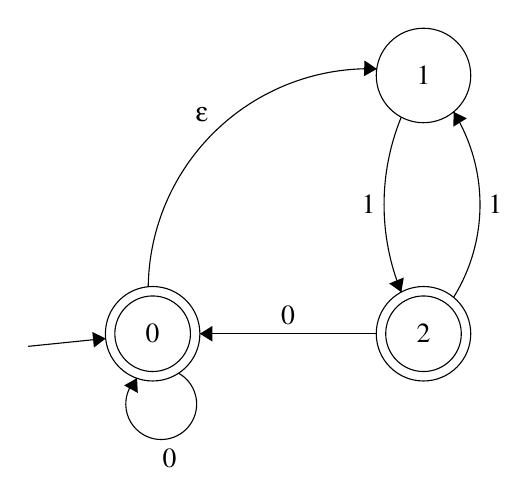
\begin{tikzpicture}[scale=0.2]
\tikzstyle{every node}+=[inner sep=0pt]
\draw [black] (24.8,-34.2) circle (3);
\draw (24.8,-34.2) node {$0$};
\draw [black] (24.8,-34.2) circle (2.4);
\draw [black] (42,-34.2) circle (3);
\draw (42,-34.2) node {$2$};
\draw [black] (42,-34.2) circle (2.4);
\draw [black] (42,-17.8) circle (3);
\draw (42,-17.8) node {$1$};
\draw [black] (26.437,-36.7) arc (60.94661:-227.05339:2.25);
\draw (25.88,-41.49) node [below] {$0$};
\fill [black] (23.81,-37.02) -- (22.99,-37.48) -- (23.86,-37.96);
\draw [black] (24.52,-31.219) arc (-180.76235:-271.96551:14.035);
\fill [black] (39.04,-17.38) -- (38.25,-16.85) -- (38.22,-17.85);
\draw (27.93,-20.77) node [above] {$\epsilon$};
\draw [black] (40.588,-31.559) arc (-157.73542:-202.26458:14.671);
\fill [black] (40.59,-31.56) -- (40.75,-30.63) -- (39.82,-31.01);
\draw (38.99,-26) node [left] {$1$};
\draw [black] (43.905,-20.106) arc (31.86937:-31.86937:11.164);
\fill [black] (43.91,-20.11) -- (43.9,-21.05) -- (44.75,-20.52);
\draw (46.09,-26) node [right] {$1$};
\draw [black] (39,-34.2) -- (27.8,-34.2);
\fill [black] (27.8,-34.2) -- (28.6,-34.7) -- (28.6,-33.7);
\draw (33.4,-33.7) node [above] {$0$};
\draw [black] (16.9,-35) -- (21.82,-34.5);
\fill [black] (21.82,-34.5) -- (20.97,-34.09) -- (21.07,-35.08);
\end{tikzpicture}
\end{center}
\item Use the subset construction method to convert your NFA to an equivalent DFA. 
Use the subsets (without the braces) to name the states in your DFA for easy grading.

\begin{center}
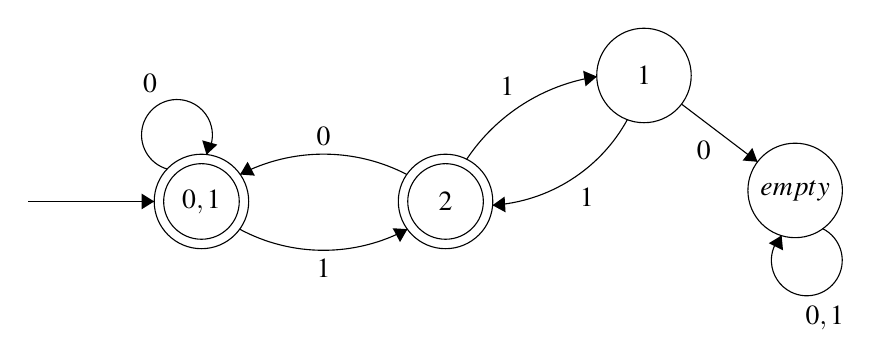
\begin{tikzpicture}[scale=0.2]
\tikzstyle{every node}+=[inner sep=0pt]
\draw [black] (20.4,-15.9) circle (3);
\draw (20.4,-15.9) node {$0,1$};
\draw [black] (20.4,-15.9) circle (2.4);
\draw [black] (35.9,-15.9) circle (3);
\draw (35.9,-15.9) node {$2$};
\draw [black] (35.9,-15.9) circle (2.4);
\draw [black] (48.5,-7.9) circle (3);
\draw (48.5,-7.9) node {$1$};
\draw [black] (58.1,-15.2) circle (3);
\draw (58.1,-15.2) node {$empty$};
\draw [black] (9.4,-15.9) -- (17.4,-15.9);
\fill [black] (17.4,-15.9) -- (16.6,-15.4) -- (16.6,-16.4);
\draw [black] (18.233,-13.842) arc (254.21614:-33.78386:2.25);
\draw (17.14,-9.04) node [above] {$0$};
\fill [black] (20.72,-12.93) -- (21.41,-12.29) -- (20.45,-12.02);
\draw [black] (33.479,-17.657) arc (-61.68386:-118.31614:11.235);
\fill [black] (33.48,-17.66) -- (32.54,-17.6) -- (33.01,-18.48);
\draw (28.15,-19.5) node [below] {$1$};
\draw [black] (22.853,-14.188) arc (117.43824:62.56176:11.495);
\fill [black] (22.85,-14.19) -- (23.79,-14.26) -- (23.33,-13.38);
\draw (28.15,-12.39) node [above] {$0$};
\draw [black] (37.239,-13.224) arc (146.30766:98.51695:12.091);
\fill [black] (45.51,-7.97) -- (44.64,-7.6) -- (44.79,-8.59);
\draw (39.82,-9.22) node [above] {$1$};
\draw [black] (47.449,-10.699) arc (-28.74082:-86.43456:10.519);
\fill [black] (38.88,-16.14) -- (39.71,-16.59) -- (39.65,-15.59);
\draw (44.87,-15.02) node [below] {$1$};
\draw [black] (50.89,-9.72) -- (55.71,-13.38);
\fill [black] (55.71,-13.38) -- (55.38,-12.5) -- (54.77,-13.3);
\draw (52.3,-12.05) node [below] {$0$};
\draw [black] (59.845,-17.626) arc (63.46232:-224.53768:2.25);
\draw (59.98,-22.52) node [below] {$0,1$};
\fill [black] (57.24,-18.06) -- (56.43,-18.55) -- (57.33,-19);
\end{tikzpicture}
\end{center}

\end{enumerate}

Collaborators: Ethan Young and Will Elliot

\item (1, 3, 3 points) Consider the NFA defined by the following transition table:

\begin{tabular}{r||c|c|c}
& $0$ & $1$ & $\epsilon$\\\hline\hline
$\rightarrow q_0$ & $\{q_2\}$ & $\emptyset$ & $\{q_1\}$\\\hline
*$q_1$ & $\{q_0\}$ & $\emptyset$ & $\emptyset$\\\hline
$q_2$ & $\{q_1\}$ & $\{q_1,q_2\}$ & $\emptyset$\\
\end{tabular}

\begin{enumerate}
\item Draw the state diagram of the NFA.

\begin{center}
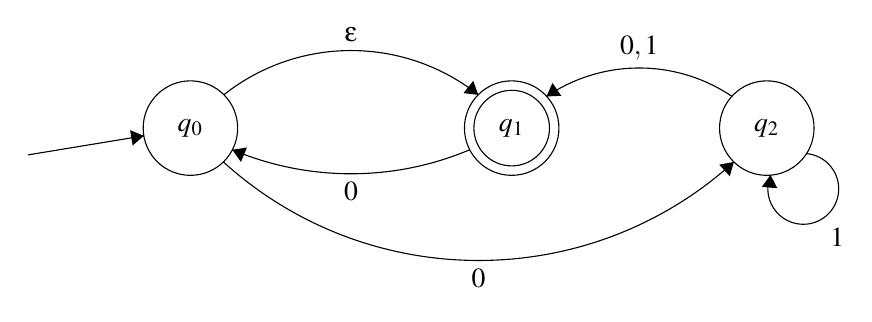
\begin{tikzpicture}[scale=0.2]
\tikzstyle{every node}+=[inner sep=0pt]
\draw [black] (12.3,-15.7) circle (3);
\draw (12.3,-15.7) node {$q_0$};
\draw [black] (32.7,-15.7) circle (3);
\draw (32.7,-15.7) node {$q_1$};
\draw [black] (32.7,-15.7) circle (2.4);
\draw [black] (48.9,-15.7) circle (3);
\draw (48.9,-15.7) node {$q_2$};
\draw [black] (14.419,-13.585) arc (128.34954:51.65046:13.025);
\fill [black] (30.58,-13.59) -- (30.26,-12.7) -- (29.64,-13.48);
\draw (22.5,-10.28) node [above] {$\epsilon$};
\draw [black] (30.037,-17.075) arc (-67.11529:-112.88471:19.382);
\fill [black] (14.96,-17.08) -- (15.51,-17.85) -- (15.89,-16.93);
\draw (22.5,-19.1) node [below] {$0$};
\draw [black] (46.809,-17.849) arc (-47.77465:-132.22535:24.119);
\fill [black] (46.81,-17.85) -- (45.88,-18.02) -- (46.55,-18.76);
\draw (30.6,-24.61) node [below] {$0$};
\draw [black] (34.912,-13.689) arc (124.09859:55.90141:10.503);
\fill [black] (34.91,-13.69) -- (35.85,-13.65) -- (35.29,-12.83);
\draw (40.8,-11.38) node [above] {$0,1$};
\draw [black] (51.413,-17.317) arc (84.96376:-203.03624:2.25);
\draw (53.37,-21.99) node [below] {$1$};
\fill [black] (49.14,-18.68) -- (48.58,-19.43) -- (49.57,-19.52);
\draw [black] (2,-17.4) -- (9.34,-16.19);
\fill [black] (9.34,-16.19) -- (8.47,-15.83) -- (8.63,-16.81);
\end{tikzpicture}
\end{center}

\item Convert the NFA to an equivalent DFA using the subsets (without the braces) to name the states in your DFA for easy grading.

\begin{center}
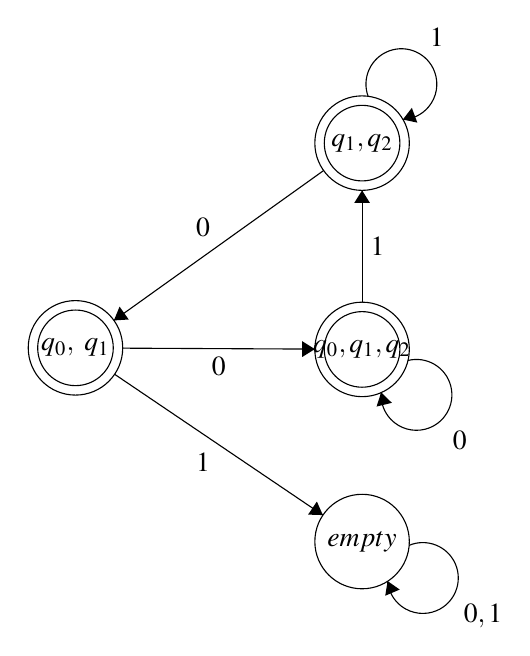
\begin{tikzpicture}[scale=0.2]
\tikzstyle{every node}+=[inner sep=0pt]
\draw [black] (14.3,-22.9) circle (3);
\draw (14.3,-22.9) node {$q_0,\mbox{ }q_1$};
\draw [black] (14.3,-22.9) circle (2.4);
\draw [black] (32.5,-23) circle (3);
\draw (32.5,-23) node {$q_0,q_1,q_2$};
\draw [black] (32.5,-23) circle (2.4);
\draw [black] (32.5,-9.9) circle (3);
\draw (32.5,-9.9) node {$q_1,q_2$};
\draw [black] (32.5,-9.9) circle (2.4);
\draw [black] (32.5,-35.2) circle (3);
\draw (32.5,-35.2) node {$empty$};
\draw [black] (17.3,-22.92) -- (29.5,-22.98);
\fill [black] (29.5,-22.98) -- (28.7,-22.48) -- (28.7,-23.48);
\draw (23.4,-23.46) node [below] {$0$};
\draw [black] (35.404,-23.704) arc (104.10996:-183.89004:2.25);
\draw (38.23,-28.77) node [right] {$0$};
\fill [black] (33.71,-25.73) -- (33.42,-26.63) -- (34.39,-26.39);
\draw [black] (32.5,-20) -- (32.5,-12.9);
\fill [black] (32.5,-12.9) -- (32,-13.7) -- (33,-13.7);
\draw (33,-16.45) node [right] {$1$};
\draw [black] (32.886,-6.937) arc (200.30993:-87.69007:2.25);
\draw (37.25,-3.78) node [above] {$1$};
\fill [black] (35.09,-8.4) -- (36.01,-8.6) -- (35.66,-7.66);
\draw [black] (30.06,-11.64) -- (16.74,-21.16);
\fill [black] (16.74,-21.16) -- (17.68,-21.1) -- (17.1,-20.28);
\draw (22.4,-15.9) node [above] {$0$};
\draw [black] (16.79,-24.58) -- (30.01,-33.52);
\fill [black] (30.01,-33.52) -- (29.63,-32.66) -- (29.07,-33.49);
\draw (22.4,-29.55) node [below] {$1$};
\draw [black] (35.478,-35.445) arc (113.03624:-174.96376:2.25);
\draw (38.93,-39.94) node [right] {$0,1$};
\fill [black] (34.12,-37.71) -- (33.97,-38.64) -- (34.89,-38.25);
\end{tikzpicture}
\end{center}

\item Describe, by filling out the blanks below, the language recognized by the FA in the form of 
$$L=\{w\in\{0,1\}^*| w {\rm\ doesn't\ start\ with\ a\  1\ and\ does\ not\ contain\ substring\ 101}\}.$$
\end{enumerate}

Collaborators: Ethan Young and Will Elliot

\item (1, 2, 3, 2 points) 

Let $L=\{w\in\{0,1\}^*\ |\ w {\rm\ doesn't\ contain\ any\ pair\ of\ 1s\ that\ are\ separated\ by\ an\ odd\ number\ of\ symbols}\}$.
\begin{enumerate}
\item Give a definition of $\overline L$.\newline 
$\overline L=\{w\in\{0,1\}^*\ |\ w {\rm\ contains\ at \ least\ one\ pair\ of\ 1s\ that\ are\ separated\ by\ an\ odd\ number\ of\ symbols}\}$.
\item Draw the state diagram of an NFA with four states that accepts $\overline L$.

\begin{center}
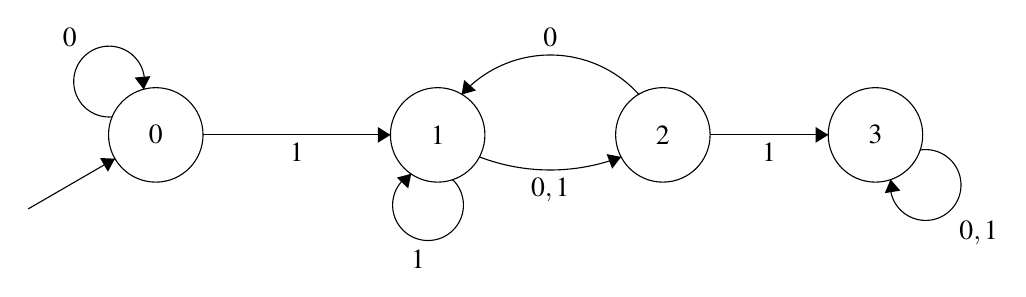
\begin{tikzpicture}[scale=0.2]
\tikzstyle{every node}+=[inner sep=0pt]
\draw [black] (14.7,-25.4) circle (3);
\draw (14.7,-25.4) node {$0$};
\draw [black] (32.6,-25.4) circle (3);
\draw (32.6,-25.4) node {$1$};
\draw [black] (46.9,-25.4) circle (3);
\draw (46.9,-25.4) node {$2$};
\draw [black] (60.4,-25.4) circle (3);
\draw (60.4,-25.4) node {$3$};
\draw [black] (11.94,-24.254) arc (275.18593:-12.81407:2.25);
\draw (9.24,-19.83) node [above] {$0$};
\fill [black] (13.93,-22.51) -- (14.36,-21.67) -- (13.36,-21.76);
\draw [black] (6.6,-30.1) -- (12.11,-26.91);
\fill [black] (12.11,-26.91) -- (11.16,-26.87) -- (11.66,-27.74);
\draw [black] (17.7,-25.4) -- (29.6,-25.4);
\fill [black] (29.6,-25.4) -- (28.8,-24.9) -- (28.8,-25.9);
\draw (23.65,-25.9) node [below] {$1$};
\draw [black] (33.545,-28.235) arc (46.16216:-241.83784:2.25);
\draw (31.35,-32.68) node [below] {$1$};
\fill [black] (30.92,-27.87) -- (30.01,-28.11) -- (30.73,-28.8);
\draw [black] (44.252,-26.796) arc (-69.03419:-110.96581:12.583);
\fill [black] (44.25,-26.8) -- (43.33,-26.62) -- (43.68,-27.55);
\draw (39.75,-28.13) node [below] {$0,1$};
\draw [black] (34.119,-22.835) arc (138.0225:41.9775:7.575);
\fill [black] (34.12,-22.84) -- (35.03,-22.58) -- (34.28,-21.91);
\draw (39.75,-19.83) node [above] {$0$};
\draw [black] (49.9,-25.4) -- (57.4,-25.4);
\fill [black] (57.4,-25.4) -- (56.6,-24.9) -- (56.6,-25.9);
\draw (53.65,-25.9) node [below] {$1$};
\draw [black] (63.23,-26.36) arc (99:-189:2.25);
\draw (65.7,-31.65) node [right] {$0,1$};
\fill [black] (61.36,-28.23) -- (60.99,-29.1) -- (61.98,-28.94);
\end{tikzpicture}
\end{center}
\item Draw the state diagram of the equivalent DFA using the subset method.

\begin{center}
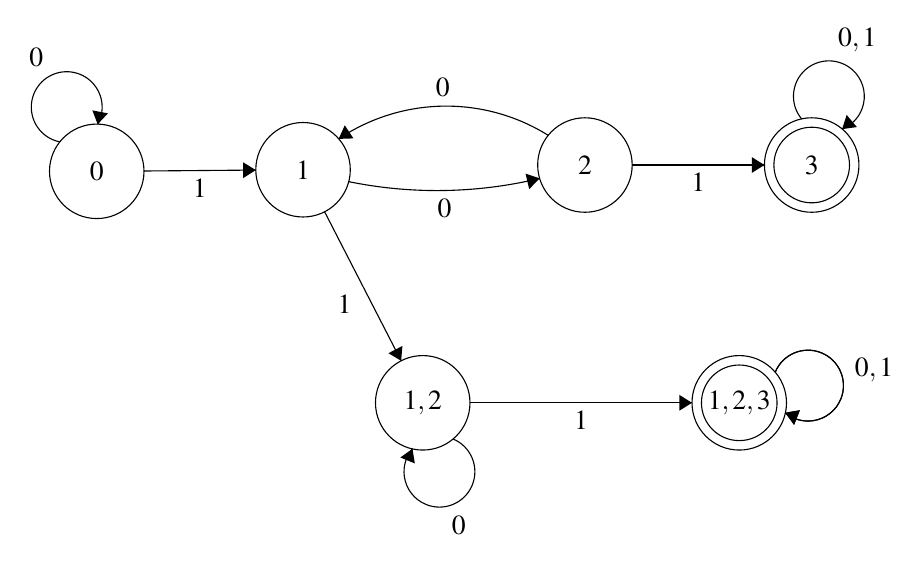
\begin{tikzpicture}[scale=0.2]
\tikzstyle{every node}+=[inner sep=0pt]
\draw [black] (11.4,-20.5) circle (3);
\draw (11.4,-20.5) node {$0$};
\draw [black] (24.5,-20.4) circle (3);
\draw (24.5,-20.4) node {$1$};
\draw [black] (42.4,-20.1) circle (3);
\draw (42.4,-20.1) node {$2$};
\draw [black] (56.8,-20.1) circle (3);
\draw (56.8,-20.1) node {$3$};
\draw [black] (56.8,-20.1) circle (2.4);


\draw [black] (32.1,-35.2) circle (3);
\draw (32.1,-35.2) node {$1,2$};
\draw [black] (52.2,-35.2) circle (3);
\draw (52.2,-35.2) node {$1,2,3$};
\draw [black] (52.2,-35.2) circle (2.4);
\draw [black] (9.067,-18.632) arc (259.05442:-28.94558:2.25);
\draw (7.56,-13.88) node [above] {$0$};
\fill [black] (11.46,-17.51) -- (12.11,-16.82) -- (11.12,-16.63);
\draw [black] (14.4,-20.48) -- (21.5,-20.42);
\fill [black] (21.5,-20.42) -- (20.7,-19.93) -- (20.7,-20.93);
\draw (17.95,-20.96) node [below] {$1$};
\draw [black] (39.525,-20.953) arc (-76.54093:-101.53873:28.013);
\fill [black] (39.53,-20.95) -- (38.63,-20.65) -- (38.86,-21.63);
\draw (33.48,-22.24) node [below] {$0$};
\draw [black] (26.761,-18.44) arc (123.90383:58.01652:12.243);
\fill [black] (26.76,-18.44) -- (27.7,-18.41) -- (27.15,-17.58);
\draw (33.38,-15.84) node [above] {$0$};
\draw [black] (45.4,-20.1) -- (53.8,-20.1);
\fill [black] (53.8,-20.1) -- (53,-19.6) -- (53,-20.6);
\draw (49.6,-20.6) node [below] {$1$};
\draw [black] (56.167,-17.18) arc (219.96376:-68.03624:2.25);
\draw (59.7,-12.93) node [above] {$0,1$};
\fill [black] (58.73,-17.82) -- (59.67,-17.69) -- (59.02,-16.92);
\draw [black] (25.87,-23.07) -- (30.73,-32.53);
\fill [black] (30.73,-32.53) -- (30.81,-31.59) -- (29.92,-32.05);
\draw (27.61,-28.93) node [left] {$1$};
\draw [black] (34.017,-37.492) arc (67.64104:-220.35896:2.25);
\draw (34.39,-42.33) node [below] {$0$};
\fill [black] (31.45,-38.12) -- (30.68,-38.67) -- (31.6,-39.05);
\draw [black] (35.1,-35.2) -- (49.2,-35.2);
\fill [black] (49.2,-35.2) -- (48.4,-34.7) -- (48.4,-35.7);
\draw (42.15,-35.7) node [below] {$1$};
\draw [black] (54.479,-33.267) arc (158.03624:-129.96376:2.25);
\draw (59.51,-33.11) node [right] {$0,1$};
\fill [black] (55.12,-35.83) -- (55.68,-36.6) -- (56.05,-35.67);
\draw [black] (54.479,-33.267) arc (158.03624:-129.96376:2.25);
\fill [black] (55.12,-35.83) -- (55.68,-36.6) -- (56.05,-35.67);
\end{tikzpicture}
\end{center}


\item Convert the above DFA to a five-state DFA that accepts $L$.
\begin{center}
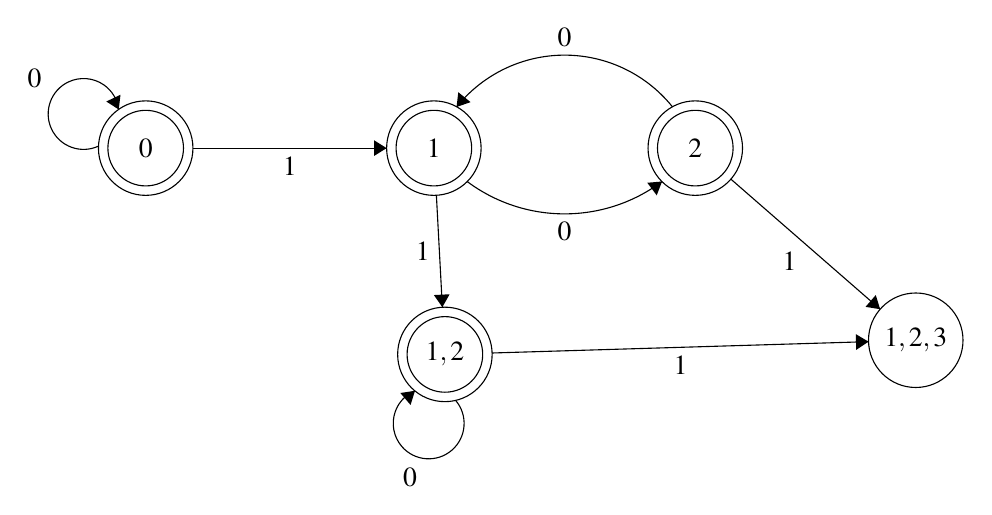
\begin{tikzpicture}[scale=0.2]
\tikzstyle{every node}+=[inner sep=0pt]
\draw [black] (9.4,-24.5) circle (3);
\draw (9.4,-24.5) node {$0$};
\draw [black] (9.4,-24.5) circle (2.4);
\draw [black] (27.7,-24.5) circle (3);
\draw (27.7,-24.5) node {$1$};
\draw [black] (27.7,-24.5) circle (2.4);
\draw [black] (28.4,-37.6) circle (3);
\draw (28.4,-37.6) node {$1,2$};
\draw [black] (28.4,-37.6) circle (2.4);
\draw [black] (44.3,-24.5) circle (3);
\draw (44.3,-24.5) node {$2$};
\draw [black] (44.3,-24.5) circle (2.4);
\draw [black] (58.3,-36.7) circle (3);
\draw (58.3,-36.7) node {$1,2,3$};
\draw [black] (6.415,-24.367) arc (295.18921:7.18921:2.25);
\draw (2.82,-20.05) node [left] {$0$};
\fill [black] (7.69,-22.05) -- (7.8,-21.11) -- (6.9,-21.54);
\draw [black] (12.4,-24.5) -- (24.7,-24.5);
\fill [black] (24.7,-24.5) -- (23.9,-24) -- (23.9,-25);
\draw (18.55,-25) node [below] {$1$};
\draw [black] (42.19,-26.618) arc (-53.21424:-126.78576:10.337);
\fill [black] (42.19,-26.62) -- (41.25,-26.7) -- (41.85,-27.5);
\draw (36,-29.18) node [below] {$0$};
\draw [black] (29.144,-21.887) arc (141.29611:38.70389:8.786);
\fill [black] (29.14,-21.89) -- (30.03,-21.58) -- (29.25,-20.95);
\draw (36,-18.09) node [above] {$0$};
\draw [black] (46.56,-26.47) -- (56.04,-34.73);
\fill [black] (56.04,-34.73) -- (55.76,-33.83) -- (55.11,-34.58);
\draw (50.29,-31.09) node [below] {$1$};
\draw [black] (31.4,-37.51) -- (55.3,-36.79);
\fill [black] (55.3,-36.79) -- (54.49,-36.31) -- (54.52,-37.31);
\draw (43.37,-37.68) node [below] {$1$};
\draw [black] (29.074,-40.511) arc (40.75948:-247.24052:2.25);
\draw (26.18,-44.75) node [below] {$0$};
\fill [black] (26.5,-39.91) -- (25.57,-40.05) -- (26.22,-40.81);
\draw [black] (27.86,-27.5) -- (28.24,-34.6);
\fill [black] (28.24,-34.6) -- (28.7,-33.78) -- (27.7,-33.83);
\draw (27.47,-31.08) node [left] {$1$};
\end{tikzpicture}
\end{center}
\end{enumerate}

Collaborators: Ethan Young and Will Elliot

\item (3, 3 points) For the following languages $A$ and $B$ over the alphabet $\{0,1\}$, prove by the closure properties that they are regular.
You are asked to use the method similar to the example given in the notes.

\begin{enumerate}
\item $A=\{w\in\{0,1\}^* | w {\rm\ contains\ neither\ the\ substrings\ } 01 {\rm\ nor\ } 10\}$

\newline $A_{1} = \{w\in\{0,1\}^* | w {\rm\ contains\ the\ substrings\ } 01 \}  $
\begin{center}
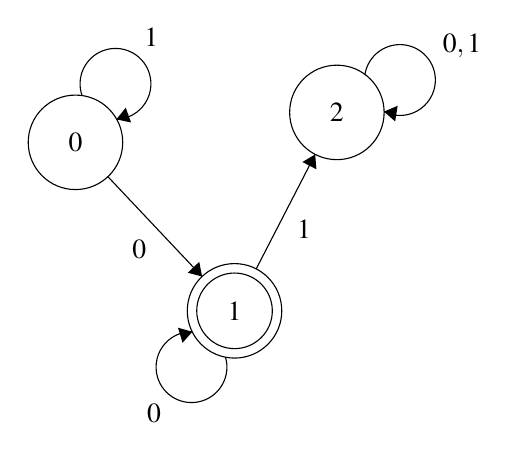
\begin{tikzpicture}[scale=0.2]
\tikzstyle{every node}+=[inner sep=0pt]
\draw [black] (14.6,-20.9) circle (3);
\draw (14.6,-20.9) node {$0$};
\draw [black] (24.7,-31.6) circle (3);
\draw (24.7,-31.6) node {$1$};
\draw [black] (24.7,-31.6) circle (2.4);
\draw [black] (31.2,-19) circle (3);
\draw (31.2,-19) node {$2$};
\draw [black] (15.022,-17.942) arc (199.61966:-88.38034:2.25);
\draw (19.41,-14.83) node [above] {$1$};
\fill [black] (17.2,-19.44) -- (18.13,-19.64) -- (17.79,-18.7);
\draw [black] (16.66,-23.08) -- (22.64,-29.42);
\fill [black] (22.64,-29.42) -- (22.46,-28.49) -- (21.73,-29.18);
\draw (19.12,-27.72) node [left] {$0$};
\draw [black] (24.123,-34.532) arc (16.59464:-271.40536:2.25);
\draw (19.59,-37.46) node [below] {$0$};
\fill [black] (22.02,-32.93) -- (21.11,-32.67) -- (21.4,-33.63);
\draw [black] (26.08,-28.93) -- (29.82,-21.67);
\fill [black] (29.82,-21.67) -- (29.01,-22.15) -- (29.9,-22.61);
\draw (28.64,-26.44) node [right] {$1$};
\draw [black] (32.98,-16.599) arc (171.18072:-116.81928:2.25);
\draw (37.89,-14.78) node [right] {$0,1$};
\fill [black] (34.19,-18.95) -- (34.9,-19.57) -- (35.06,-18.58);
\end{tikzpicture}
\end{center}

\newline 
\newline $A_{2} = \{w\in\{0,1\}^* | w {\rm\ contains\ the\ substrings\ } 10 \}  $

\begin{center}
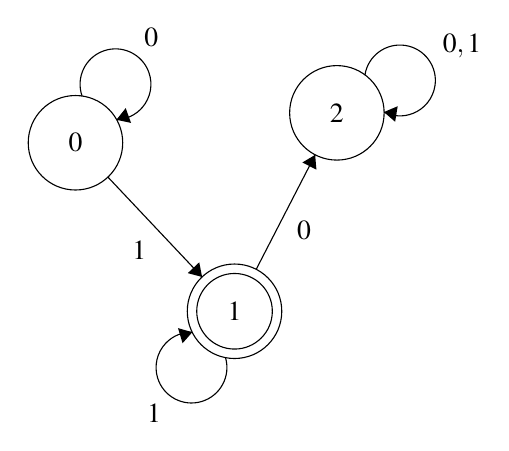
\begin{tikzpicture}[scale=0.2]
\tikzstyle{every node}+=[inner sep=0pt]
\draw [black] (14.6,-20.9) circle (3);
\draw (14.6,-20.9) node {$0$};
\draw [black] (24.7,-31.6) circle (3);
\draw (24.7,-31.6) node {$1$};
\draw [black] (24.7,-31.6) circle (2.4);
\draw [black] (31.2,-19) circle (3);
\draw (31.2,-19) node {$2$};
\draw [black] (15.022,-17.942) arc (199.61966:-88.38034:2.25);
\draw (19.41,-14.83) node [above] {$0$};
\fill [black] (17.2,-19.44) -- (18.13,-19.64) -- (17.79,-18.7);
\draw [black] (16.66,-23.08) -- (22.64,-29.42);
\fill [black] (22.64,-29.42) -- (22.46,-28.49) -- (21.73,-29.18);
\draw (19.12,-27.72) node [left] {$1$};
\draw [black] (24.123,-34.532) arc (16.59464:-271.40536:2.25);
\draw (19.59,-37.46) node [below] {$1$};
\fill [black] (22.02,-32.93) -- (21.11,-32.67) -- (21.4,-33.63);
\draw [black] (26.08,-28.93) -- (29.82,-21.67);
\fill [black] (29.82,-21.67) -- (29.01,-22.15) -- (29.9,-22.61);
\draw (28.64,-26.44) node [right] {$0$};
\draw [black] (32.98,-16.599) arc (171.18072:-116.81928:2.25);
\draw (37.89,-14.78) node [right] {$0,1$};
\fill [black] (34.19,-18.95) -- (34.9,-19.57) -- (35.06,-18.58);
\end{tikzpicture}
\end{center}

\newline Since both $A_{1}$ and $A_{2}$ are regular languages, the intersection between the two languages will also be a regular language given by the closure property. Therefore A is a regular language. 
\item $B=\{w\in\{0,1\}^* | w {\rm\ contains\ at\ least\ two\ 0's\ and\ at\ most\ one\ 1}\}$ \newline 

$B_{1} =\{w\in\{0,1\}^* | w {\rm\ contains\ at\ least\ two\ 0's\}\}$
\begin{center}
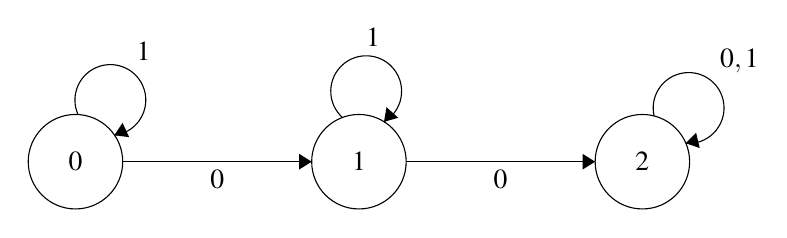
\begin{tikzpicture}[scale=0.2]
\tikzstyle{every node}+=[inner sep=0pt]
\draw [black] (11,-20.3) circle (3);
\draw (11,-20.3) node {$0$};
\draw [black] (29,-20.3) circle (3);
\draw (29,-20.3) node {$1$};
\draw [black] (47,-20.3) circle (3);
\draw (47,-20.3) node {$2$};
\draw [black] (11.169,-17.316) arc (204.4867:-83.5133:2.25);
\draw (15.32,-13.92) node [above] {$1$};
\fill [black] (13.47,-18.62) -- (14.41,-18.74) -- (13.99,-17.83);
\draw [black] (14,-20.3) -- (26,-20.3);
\fill [black] (26,-20.3) -- (25.2,-19.8) -- (25.2,-20.8);
\draw (20,-20.8) node [below] {$0$};
\draw [black] (27.959,-17.499) arc (228.12402:-59.87598:2.25);
\draw (29.89,-13) node [above] {$1$};
\fill [black] (30.59,-17.77) -- (31.5,-17.51) -- (30.75,-16.84);
\draw [black] (32,-20.3) -- (44,-20.3);
\fill [black] (44,-20.3) -- (43.2,-19.8) -- (43.2,-20.8);
\draw (38,-20.8) node [below] {$0$};
\draw [black] (47.746,-17.406) arc (193.27825:-94.72175:2.25);
\draw (53.16,-14.69) node [above] {$0,1$};
\fill [black] (49.75,-19.13) -- (50.64,-19.43) -- (50.41,-18.46);
\end{tikzpicture}
\end{center}

\newline 
$B_{2} =\{w\in\{0,1\}^* | w {\rm\ contains\ at\ most\ one\ 1}\}$
\begin{center}
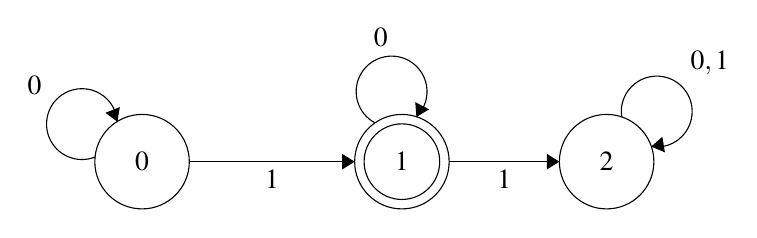
\begin{tikzpicture}[scale=0.2]
\tikzstyle{every node}+=[inner sep=0pt]
\draw [black] (10.8,-23.6) circle (3);
\draw (10.8,-23.6) node {$0$};
\draw [black] (27.3,-23.6) circle (3);
\draw (27.3,-23.6) node {$1$};
\draw [black] (27.3,-23.6) circle (2.4);
\draw [black] (40.3,-23.6) circle (3);
\draw (40.3,-23.6) node {$2$};
\draw [black] (7.827,-23.301) arc (291.99462:3.99462:2.25);
\draw (4.45,-18.73) node [left] {$0$};
\fill [black] (9.23,-21.06) -- (9.39,-20.13) -- (8.47,-20.5);
\draw [black] (25.602,-21.141) arc (242.35527:-45.64473:2.25);
\draw (25.96,-16.33) node [above] {$0$};
\fill [black] (28.22,-20.76) -- (29.03,-20.28) -- (28.15,-19.82);
\draw [black] (13.8,-23.6) -- (24.3,-23.6);
\fill [black] (24.3,-23.6) -- (23.5,-23.1) -- (23.5,-24.1);
\draw (19.05,-24.1) node [below] {$1$};
\draw [black] (30.3,-23.6) -- (37.3,-23.6);
\fill [black] (37.3,-23.6) -- (36.5,-23.1) -- (36.5,-24.1);
\draw (33.8,-24.1) node [below] {$1$};
\draw [black] (41.26,-20.77) arc (189:-99:2.25);
\draw (45.6,-17.35) node [right] {$0,1$};
\fill [black] (43.13,-22.64) -- (44,-23.01) -- (43.84,-22.02);
\end{tikzpicture}
\end{center}
\end{enumerate}

\newline Since both $B_{1}$ and $B_{2}$ are regular languages, the intersection between the two languages will also be a regular language given by the closure property. Therefore B is a regular language. 

Collaborators: Ethan Young and Will Elliot

\end{enumerate}

\end{document}